\documentclass[10pt]{article}

\usepackage{commands}

\begin{document}
\begin{tcolorbox}
  \begin{center}
  \begin{Large}
    \textbf{Physics 474 – Applied Solid State Physics - Course Notes} \\
    \vspace{5pt}
  \end{Large}
  \begin{large}
        Tobias Faehndrich \\
\vspace{5pt}
    \emph{This document was typeset on \today}
  \end{large}
  \end{center}
\end{tcolorbox}

\begin{center}
  \textbf{Introduction:}

Notes written while following Dr. Alannah Hallas's PHYS 474 UBC lecture notes. If any errors are found in the notes, feel free to email me at \href{mailto:tobias.faehndrich@gmail.com}{tobias.faehndrich@gmail.com}. Overleaf formatting was copied from Rio W.

\end{center}
\addtocontents{toc}{\protect\hypertarget{toc}{}}
\tableofcontents

\newpage
\section[Introduction]{\hyperlink{toc}{Introduction}}

This lecture talked about the course structure, grading and basic questions about solid state physics and why it is important.



\newpage
\input{Lectures/02 Heat Capacity Models I — Boltzmann and Einstein}


\newpage
\input{Lectures/03 Heat Capacity Models II — Einstein Revisited and Debye}

\newpage
\section[Heat Capacity Models III — Drude Model]{\hyperlink{toc}{Heat Capacity Models III — Drude Model}}

Recall:
\textbf{The Density of states}

\begin{itemize}
    \item It is conventional to express integrals of this type in terms of the density of states, $g(\omega)$, which is defined as the number of states per unit frequency interval, i.e.,
    \[ \avg{E} = \int_{0}^{\infty} \dd{\omega} \, g(\omega) \, \hbar \omega \brackets*{\frac{1}{e^{\beta \hbar \omega} - 1} + \frac{1}{2}} \]


    where $\beta = \frac{1}{k_B T}$, and $k_B$ is the Boltzmann constant.
    \[ g(\omega) = L^3 \frac{12 \pi \omega^2}{(2 \pi)^3 v^3} \]

    \item The density of states tells us how many new modes (sound waves here) are available at a given temperature / frequency ($\hbar \omega = k_B T$).

    \item The DOS for the Einstein model would look like a delta function at $\omega = \omega_E$.
    \item The DOS for the Debye model is a parabola ($g(\omega) \propto \omega^2$), which is a good approximation for low frequencies.

    \item Solving for the integral for $\avg{E}$ (as done in HW \#1) gives:
    
    \[ \avg{E} \propto \text{T-independent} + a \text{T}^4 \]

    where the T-independent term is the zero-point energy, and the $a \text{T}^4$ term is the contribution from the phonons. a being some constant.

    \item The low T limit accounts for the $T^3$ law
    
    \[ \dv{\avg{E}}{T} = C \propto a \text{T}^3 \]

    which agrees with experiment.

    \item The high T limit does not saturate at the Dulong-Petit Law value,
    
    \[ C \propto a \text{T}^3 \]

    still at all temperatures, and never saturates to the Dulong-Petit Law value of $3Nk_B$.
    
    \item Dybye comes up with a solution to this problem, imposing that there should only be as many modes as there are degrees of freedom, i.e. integrate between $0$ and $\omega_{\text{cutoff}}$
    
    \[ 3N = N_{\text{atoms}} \cdot 3 = \# \text{ allowed modes} \]
    
    This was built into Einstein's calculation.

    \[ 3 N = \int_{0}^{\omega_{\text{cutoff}}} \dd{\omega} \, g(\omega) \]

    then evaluate this integral to find the cutoff frequency, $\omega_{\text{cutoff}}$.

    \item This now gives the correct high T limit agreeing with the Dulong-Petit Law:
    \[ \avg{E} = \int_{0}^{\omega_{\text{cutoff}}} \dd{\omega} \, g(\omega) \, \hbar \omega \brackets*{\frac{1}{e^{\beta \hbar \omega} - 1} + \frac{1}{2}} \Rightarrow 3 R T \, \text{as} \, T \to \infty \]

    where $R$ is the gas constant, and $3 R$ is the Dulong-Petit Law value.

    \item This cutoff frequency is the Debye frequency, $\omega_D$, and the Debye temperature is defined as:

    \[ \omega_{\text{cutoff}} = \omega_D = \sqrt[3]{\frac{6 \pi^2 N^3}{V^3}}  = \sqrt[3]{6 \pi^2 n v^3}\]

    where $n$ is the number density of atoms ($n = \frac{N}{V}$), and $v$ is the speed of sound in the material.

    \item $T_D$ is the Debye temperature (also called $\theta_D$)
    \[ T_D = \frac{\hbar \omega_D}{k_B} \]
    
    \item If a material undergoes a phase transition causing its colume to half. What will happen to the Debye temperature? (assume $v$ is constant - is this a good assumption?)
    
    \begin{itemize}
        \item $T_D = \frac{\hbar \omega_D}{k_B} = \frac{\hbar}{k_B} \sqrt[3]{6 \pi^2 n v^3}$
        \item $n$ will double, so $T_D$ will increase by a factor of $\sqrt[3]{2}$.
        \item If the speed of sound is not constant, then the change in $T_D$ will depend on how the speed of sound changes with volume.
    \end{itemize}

    \item Debye and Einstein are similar, but Debye model is more accurate for low temperatures.
    
    \item Note that at intermediate temperatures, the integral in the Debye formulation can only be solved numerically.
    
    \item Debye model \underbar{very} successful, but not perfect:
    \begin{itemize}
        \item Less accurate at intermediate temperatures.
        \item Introduciton of $\omega_{\text{cutoff}}$ is somewhat arbitrary.
        \item Assumption of $\omega=vk$ becomes questionable for short wavelengths (high frequencies).
        \item Metals have an additional T-linear contribution to C that is missed by the Debye model.
    \end{itemize}
    
\end{itemize}


\subsection{Drude Theory (Chapter 3)}

\begin{itemize}
    \item So far, we've talked about atomic vibrations (effectively, a property of the nucleus). next we are going to talk about the conduction of electricity (a property of the electrons).
    \item What we already know from real life: some materials conduct electricity and are therefrore metals, and others do not. We are going to skip over (for now) what makes a material a metal and jump straight into understanding the properties of the conduction electrons.
    \item Basic idea: Drude (Drew-duh) extended Boltzmann's kinetic theory of gases (see the ideal gas law) to the motion of electrons in a metal (no atoms, just a gas of electrons).
\end{itemize}

\textbf{Assumptions of the Drude model}
\begin{itemize}
    \item The basic assumptions of the Drude model are:
    \begin{enumerate}
        \item The electrons have some characteristic scattering time, $\tau$ (material dependent, average time between collisions). The probability of scattering in a time interval $dt$ is $P = \frac{dt}{\tau}$. (reasonable. note that it assumes nothing about nature of scattering).
        \item After scattering, the electron has zero kinetic energy (i.e. $\vec{p} = 0$). This is questionable, but true on average.
        \item The electrons will respond to externally applied electric and magnetic fields. This is reasonable, electrons are charged.
    \end{enumerate}
\end{itemize}


\textbf{Equation of motion for the Drude Model}
\begin{itemize}
    \item In order to understand the behaviour of the conduction electrons, we will start by defining the average momentum for an electron, which depends on whether or not it experienced a scattering event.
    
    time $dt$ later: 
    \[
    \begin{aligned}
    \avg{\vec{p}(t+dt)} &= \Prob_{\text{no scatter}} \cdot \vec{p}_{\text{no scatter}} + \Prob_{\text{scatter}} \cdot \vec{p}_{\text{scatter}} \\
    &= \paren*{1-\frac{dt}{\tau}} \cdot \paren*{\vec{p}(t) + \vec{F}dt} + \paren*{\frac{dt}{\tau}} \cdot 0
    \end{aligned}
    \]

    where $d\vec{p} = \vec{F} dt $ and Lorentz force $\vec{F} = -e (\vec{E} + \vec{v} \times \vec{B})$

    \[ \avg{\vec{p}(t+dt)} = \vec{p}(t)-\frac{\vec{p}(t) dt}{\tau} + \vec{F}dt - \frac{\vec{F} dt^2}{\tau} \]


    \item For $dt \ll 1$, we can keep only terms that are of first-order in $dt$:
    
    We get an equation of motion!
    \[ \boxed{\frac{d\vec{p}}{d\tau} = \vec{F} - \frac{\vec{p}(t)}{\tau}} \]

    last term acts like a drag forc on the electron.
    
    \item What does this give in the absence of any applied field? Does that make sense?
    
    \[ \vec{F} = 0 \Rightarrow \frac{d\vec{p}}{d\tau} = -\frac{\vec{p}(t)}{\tau} \]

    \[ \vec{p}(t) = \vec{p}(0) \cdot \e^{-\frac{t}{\tau}} \]

    which gives an expenential decay of the momentum of the electron to zero. In the model this makes sense, but in real life this is not the case.
    
\end{itemize}










\newpage
\section[Electrical conductivity and the Hall effect]{\hyperlink{toc}{Electrical conductivity and the Hall effect}}


\subsection{Electrical conductivity in the Drude model}

\begin{itemize}
    \item Next, let's consider when we have a non-zero electrical field (with $\mathbf{B}$ still 0):
    
    \[ \vec{E} \neq 0, \quad \vec{B} = 0 \]

    Equation of motion:

    \[ \dv{\vec{p}}{t} = -e \vec{E} - \frac{\vec{p}(t)}{\tau} \]

    \item We can now define the conductivity of a metal, $\sigma$, which is the constant of proportionality between the current density $\vec{j}$, and the applied electric field $\vec{E}$.
    
    \begin{center}
        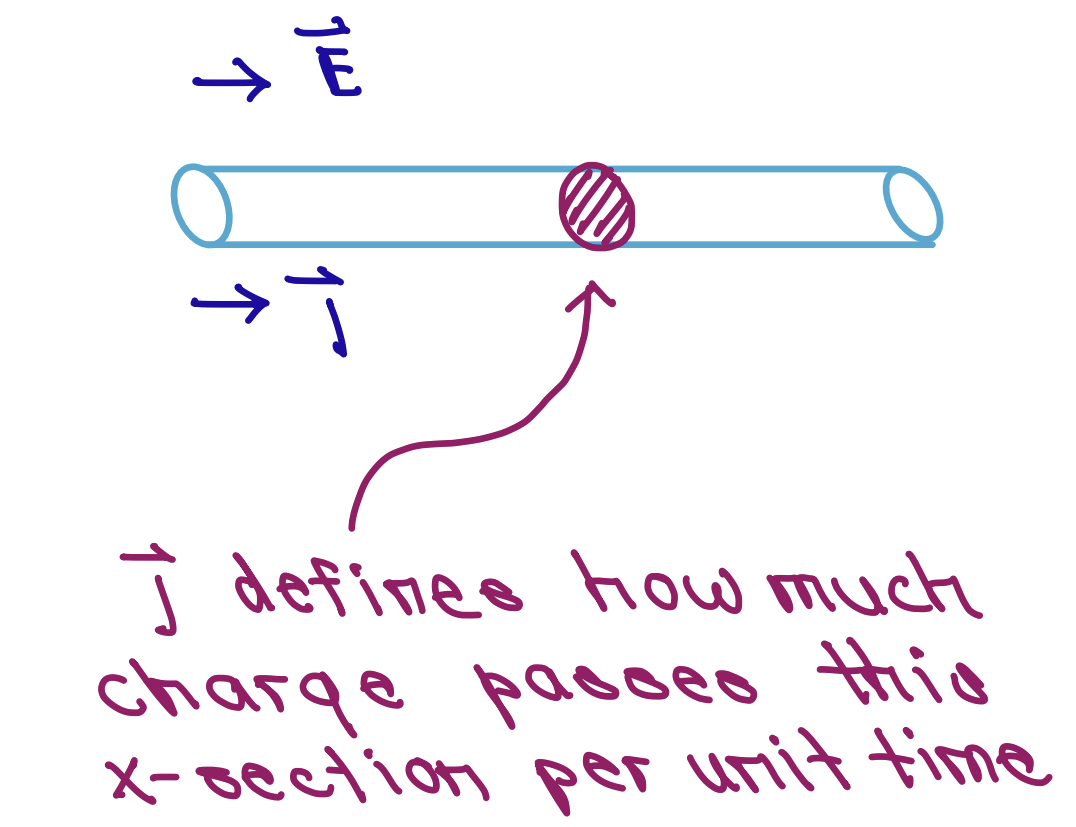
\includegraphics[width = 0.3 \linewidth]{Images/current-density.png}
    \end{center}

    where

    \[\vec{j} = \text{current density} \]
    
    which is the charge per unit time per unit area

    \[ \vec{j} = - n e \vec{v} \]

    where $n$ is the density of electrons   

    \[ \brackets*{e^-/m^3}\brackets*{C/e^-} \brackets*{m/s} = \frac{C}{m^2 \cdot s} \]

    \[ \vec{j} = \frac{e^2 n \tau}{m} \vec{E} \Rightarrow \boxed{\sigma = \frac{e^2 n \tau}{m}} \text{ units } \brackets*{\Omega^{-1} m^{-1}}\]

    \item Thus we can define resistivity $\rho$ as the inverse of conductivity:
    
    \[ \boxed{\rho = \frac{1}{\sigma} }  \text{ units } \brackets*{\Omega m}\]

    \item If the resistivity of a metal is given by $\rho = \frac{1}{\sigma} = \frac{m}{e^2 n \tau}$, then decreasing the collision rate ($\frac{1}{\tau}$), will increase $\tau$ and thus lower the resistance.
    
    \item Note that increasing or decreasing the size of the sample does not change the resistivity. $\rho$ is \emph{intrinsic} (depends on material properties), while $R= \rho \cdot \frac{L}{A}$ is \emph{extrinsic} (depends on the size and shape of the sample).

    \item \[ \sigma \propto \tau \Rightarrow \uparrow \tau \text{ means fewer collisions per electron (lower collision rate)} \]
\end{itemize}

\subsection{Hall Effect}
\begin{center}
    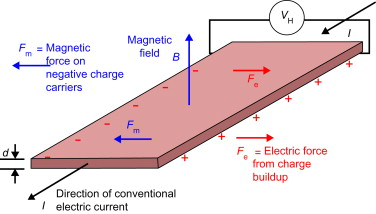
\includegraphics[width = 0.4 \linewidth]{Images/hall-effect.jpg}
\end{center}

\begin{itemize}

    \item Next, we can apply an electric and magnetic field to our metal simultaneously (in perpendicular directions). By convention, we will always apply $\mathbf{B}$ in the $z$ direction. 
    
    \item Recall -- equation of motion:
    
    \[ \dv{\vec{p}}{t} = -e \left( \vec{E} + \vec{v} \times \vec{B} \right) + \frac{\vec{p}(t)}{\tau} \]

    \item If we again assumee steady state, we get:
    \[ \vec{E} = \left( \frac{m}{ne^2 \tau} \right) \vec{j} + \left( \frac{1}{ne} \right) \vec{j} \times \vec{B} \]

    where the first term is "longitudinal"  and the second term is off diagonal.

    \item We can define a 3 x 3 resistivity matrix and we find that the application of a $\mathbf{B}$ field deflects the electrons causing a measurable potential difference in the orthogonal direction -- this is the Hall effect.
    
    \[ \vec{B} \parallel \hat{z}, \quad \vec{j} \text{ can be applied along } \hat{x}, \hat{y}, or \hat{z} \]
        
    \[ \rho_{xx} = \rho_{yy} = \rho_{zz} = \frac{m}{ne^2 \tau} \]

    Hall resistivity:

    \[ \boxed{ \rho_{xy} = -\rho_{yx} = \frac{B}{ne}} \]

    \item Note that in steady state the current flows in only one spatial direction.
    
    \begin{itemize}
        \item In the steady state, once the potential difference is established in the transverse direction, no additional current flows in that direction.
        \[ \text{i.e.} \quad |\vec{F}_{\text{e}}| = |\vec{F}_{\text{B}}| \quad \text{ on the previous diagram} \]

        
        \item current only flows in the "applied" direction.
    \end{itemize}

    \item KEY! Whereas the longitudinal resistivity ($\rho_{xx}$) depends on both $\tau$ and $n$ -- so that they cannot be uniquely determined -- \textbf{the Hall resistivity depends only on n}, so we can determine the number of conduction electrons. 
    \item We can define the Hall coefficient, $R_H$:
    \[ R_H = \frac{-1}{ne} = \frac{-\rho_{xy}}{|B|} \quad \text{ units } \brackets*{m^3/C}\]

    note: "normal" meteals have a negative $R_H$ (NOT a resistance).

    \begin{center}
        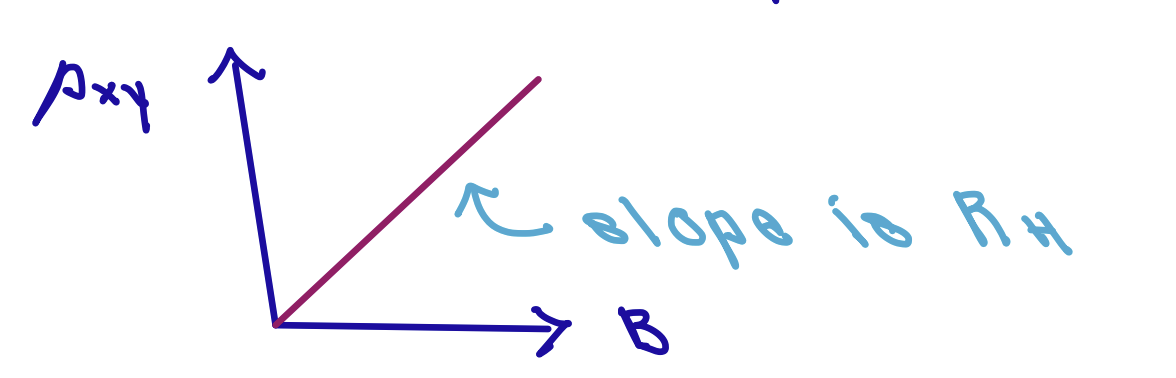
\includegraphics[width = 0.4 \linewidth]{Images/hall-effect-slope.png}
    \end{center}

    \item Some metals have a positive Hall coefficient -- seeming to imply the existence of a positively charged carrier of electrical current. This is forshadowing for later in the course when we will get introduced to the concept of holes in semiconductors.

    \item The Hall coefficient $R_H$ for copper (good metal) is of order 0.1 $mm^3/C$ and its resistivity at RT is of order $10^{-8} \Omega m$. The order of magnitude of the scattering time, $\tau$.
    
    \[ R_H = 0.1 mm^3/C = 10^{-10} m^3/C = \frac{-1}{n e} \]

    \[ \rho = \frac{1}{\sigma} = 10^{-8} \Omega m = \frac{m}{n e^2 \tau} \]

    \[ \tau = \frac{-m R_H}{e^2 \rho} = \frac{-\paren*{10^{-30}\, \text{kg}} \paren*{10^{-10} m^{3}/C}}{\paren*{-10^{-19} C} \paren*{10^{-8} \Omega m}} = 10^{-13} s \]

    \item Average metal $\approx$ 10$^{-14}$ s, so this is reasonable. Scattering time is extraordinarile short. 
\end{itemize}

\end{document}